\chapter{METHODOLOGY}
\section{Process Model}
In this project, we opted to follow agile model\cite{agile} since we felt it was the best way of going forward learning the technology, easier way of learning together and is used during production on companies. Since in this model we can build  our application in various iterations, working application features needed later on if found important could be integrated easily. This model also promotes teamwork and allow for cross-training i.e. allows us to go on with our plan of making both web application through React Js. and Android Application through Flutter. Debugging should also be easier using this model since at the beginning small application of doing main task of booking the room could be developed then including the other parts on later iterations making it easier and helping to find out the bug on the software quicker. Documentation could also be done easily which is important since the project is to be done in such time constraint. 
\begin{figure}[ht]
	\centering
	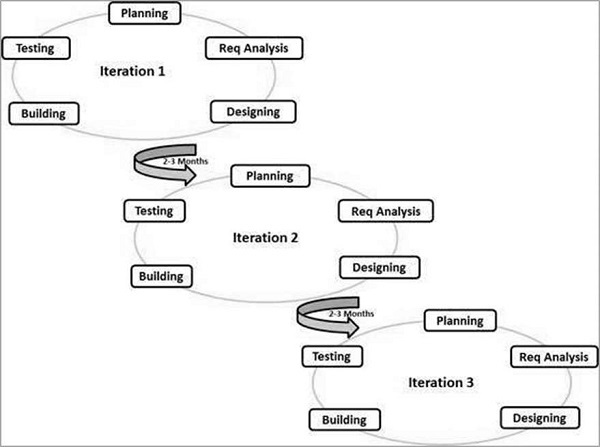
\includegraphics[width=\linewidth,height=250px]{Graphics/sdlc_agile_model.jpg}
	\caption{Agile Model\cite{agile} }
\end{figure}

\section{Tools to be used}

\subsection{Android}
Android is an Linux kernel based mobile operating system managed by Google. It is used by several smartphones and tablets. Example includes Samsung Galaxy, OnePlus, etc. \\
Unlike Apple's iOS, Android is an open source i.e. developer can modify or customize the OS for each phone. Even this is the case, application on similar android version can run on all the platform regradless of the vendor of the phone and unlike iOS, application can be deployed for testing and presenting purpose on an actual phone though any PC while iOS needs a MAC.

\subsection{Android Studio}
Android Studio is an official Integrated Development Environment(IDE) for Android, based on IntelliJ IDEA. On top of IntelliJ's powerful code editor and developer tools, Android Studio even offers more features that enhances your productivity with building Android Application.\\
Virtual android device is one of the important features which allow testing of files in different virtual android devices. Using developer mode's USB debugging mode feature.

\subsection{VSCode}
Visual Studio Code is a lightweight but powerful source code editor.  It comes with built-in support for JavaScript, TypeScript and Node.js and has a rich ecosystem of extensions for other languages (such as C++, C\#, Java, Python, PHP, Go) and runtimes (such as .NET and Unity).\\
This IDE also allow android application development though testing in users mobile through the developer mode's USB debugging mode feature.
\subsection{Flask}
Flask is an microframework made from Python. Here the word 'micro' doesn't mean that it lacks functionality but is simple in it's core but is extensible. Decisions such as which database to use is not decided by flask and decisions of flask such as it's template engine of Jinja can be changed easily. 
\subsection{React Js.}
React is a JavaScript library for building user interfaces. React has been designed from the start for gradual adoption, and you can use as little or as much React as you need.
\subsection{Flutter}
Flutter is Google’s UI toolkit for building beautiful, natively compiled applications for mobile, web, and desktop from a single codebase. In it's core, it uses dart programming language. It has features of fast development, good native performance with expressive and flexible UI.
\subsection{PostgreSQL}
PostgreSQL is a powerful, open source object-relational database system that uses and extends the SQL language combined with many features that safely store and scale the most complicated data workloads.\\
PostgreSQL has earned a strong reputation for its proven architecture, reliability, data integrity, robust feature set, extensibility, and the dedication of the open source community behind the software to consistently deliver performance and innovative solutions. PostgreSQL runs on all major operating systems, has been ACID-compliant since 2001, and has powerful add-ons such as the popular PostGIS geospatial database extender.\\
\subsection{SQLAlchemy}
SQLAlchemy is the Python SQL toolkit and Object Relational Mapper that gives application developers the full power and flexibility of SQL.\\
It provides a full suite of well known enterprise-level persistence patterns, designed for efficient and high-performing database access, adapted into a simple and Pythonic domain language.
\section{Block Diagram}
\begin{figure}[ht]
	\centering
	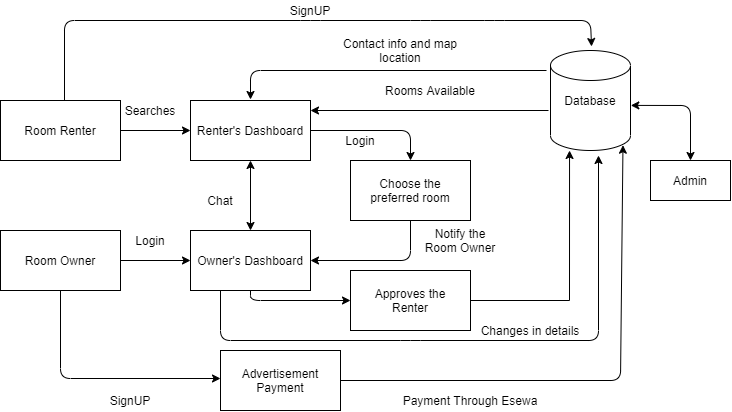
\includegraphics[width=\linewidth, height=250px]{Graphics/diagram.png}
	\caption{System Block Diagram }
\end{figure}
When room renter opens the application an interface which allows the user to check rooms available. In order to choose the room they prefer login is needed and if there is no account then room renter has to signup. After the room renter has signed in and choosen there prefered room, notification is sent to the room owner. \\
When Room Owner opens the application, owner has to signup initally and choose advertisement plan then do online payment through the application. Next time they can just login then be presented to owner's dashboard where they can update more information about their room. If renter chooses their room then they can chat with the room renter.\\
After chatting through the application, if both come to an agreement, owner can then share their number and location by approving the renter. Renter can then find the rented room through the Google Map route from the application.\\
Admin can review all the transactions and could change data in database for improvement.\\
\section{Algorithm}
\begin{algorithm}[H]
	Step1: Looks for the content \\
	Step2:\While{User Finds proper room or exits}{
	Step3: \uIf{User Logged in}{
				Goto Step6
			}
			\uElseIf{User account exists}{
				Goto Step5
			}
			\uElse{
				Goto Step4
			}
	Step4: Signup for new account\\
	Step5: Login\\
	Step6: Choose Preferred room(Notification is sent to the Room owner)\\
	Step7: Chatting with the Room owner through the application\\
	Step8: \uIf{Room Owner Agrees}{
				Recieves detail i.e. Map and contact info.
			}\uElse{
				Recieves info that the request has been denied.
			}
	}
	\caption{For Room Renter}
\end{algorithm}
This Algorithm shows how a room renter can use our application.\\
\begin{algorithm}[H]
	Step1: \uIf{User Logged in}{
				Goto Step4
			}
			\uElseIf{User account exists}{
				Goto Step3
			}
			\uElse{
				Goto Step2
			}
	Step2: Signup for new account\\
	Step3: Registers for Advertisement\\
	Step4: Login\\
	Step5: \uIf{User want to change detail}{
				Change detail
			}
	Step6: \While{No requests}{
				No requests
			}
	Step7: Chatting with the Room Renter through the application.
	Step8: \uIf{Approves}{
				Goto Step9
			}
			\uElse{
				Rejects the applicant and they get the information\\
				Goto Step6
			}
	Step9: Option of sending phone number, Location of the house through maps.
	\caption{For Room Owner}
\end{algorithm}
This Algorithm shows how a room owner can use our application.
